\documentclass[main.tex]{subfiles}
\begin{document}

\section{Argument Structure}

The classification systems discussed in this section considered the argument structure of verbs. In general, every finite verb in English takes one or more arguments, with a subject argument being required in normal speech and writing. The Stanford NLP system marks the arguments of verbs using the dependencies shown in Table~\ref{table:arg-deps}. In the majority of non-copular sentences, the governors of these dependencies are the core verbs. In copular sentences the governor is generally the subject complement (i.e. the argument generally appearing after the verb which is equated with the subject) though in the case of copular sentences with clausal subjects, the Stanford parser chooses the copula to be the governor.
Figure~\ref{ex:arg-deps} show examples of these dependencies.

\begin{table}[ht]
\small
\centering
\caption{The dependencies used to identify verbal arguments.}
\begin{tabular}{ l l }
\toprule
ccomp & Clausal Complement\\
csubj & Clausal Subject\\
csubjpass & Passive Clausal Subject\\
dobj & Direct Object\\
iobj & Indirect Object \\
nsubj & Nominal Subject\\
nsubjpass & Passive Nominal Subject\\
xcomp & Open Clausal Complement\\

\bottomrule
\end{tabular}
\label{table:arg-deps}
\end{table}

\begin{figure}[ht]
\caption{Examples of the Dependencies Listed in Table~\ref{table:arg-deps}. \textit{a}, native sample from ICE-CAN; \textit{b,c,d}, native samples from MICUSP; \textit{e,f} from \citet{typed-deps-manual}.}

\centering
\begin{tabular}{ l l }
%ICE Canada
a. &
\xytext{
\xybarnode{In} &
\xybarnode{nineteen} &
\xybarnode{ninety-seven} &
\xybarnode{Roland} &
\xybarnode{Lemon} &
\xybarnode{was} &
\xybarnode{elected} 
\xybarconnect(U,U){-2}"_{\small nsubjpass}"
\xybarconnect(D,D){1}"_{\small dobj}"
&
\xybarnode{president.} 
}\\

b. &
%MICUSP native
\xytext{
\xybarnode{\ldots} &
\xybarnode{before} &
\xybarnode{his} &
\xybarnode{father} &
\xybarnode{gave} 
\xybarconnect(UL,U){-1}"_{\small nsubj}"
\xybarconnect(UR,U){1}"^{\small iobj}"
\xybarconnect(D,D){3}"_{\small dobj}"&
\xybarnode{him} &
\xybarnode{the} &
\xybarnode{rest} &
\xybarnode{of} &
\xybarnode{it.}
}\\
%MICUSP native
c. &
\xytext{
\xybarnode{They} &
\xybarnode{state} 
\xybarconnect(U,U){-1}"_{\small nsubj}"
\xybarconnect(D,D){3}"_{\small ccomp}"&
\xybarnode{that} &
\xybarnode{climate} &
\xybarnode{generally} &
\xybarnode{predicts} 
\xybarconnect(U,U){-2}"_{\small nsubj}"
\xybarconnect(D,D){4}"_{\small ccomp}"&
\xybarnode{that} &
\xybarnode{temperatures} &
\xybarnode{should} &
\xybarnode{rise}
\ldots
}\\

%MICUSP native
d. &
\xytext{
\xybarnode{Before} &
\xybarnode{Yeltsin} &
\xybarnode{appointed} 
\xybarconnect(U,U){-1}"_{\small nsubj}"
\xybarconnect(D,D){5}"_{\small xcomp}"&
\xybarnode{him} &
\xybarnode{the} &
\xybarnode{deputy} &
\xybarnode{Prime} &
\xybarnode{Minister}
\xybarconnect(U,U){-4}"_{\small nsubj}"&
\ldots
}\\

%Dep Manual
e. &
\xytext{
\xybarnode{That} &
\xybarnode{she} &
\xybarnode{lied} 
\xybarconnect(U,U){-1}"_{\small nsubj}"&
\xybarnode{was} &
\xybarnode{suspected}
\xybarconnect(D,D){-2}"^{\small csubjpass}"&
\xybarnode{by} &
\xybarnode{everyone.}
}\\
%Dep manual
f. &
\xytext{
\xybarnode{What} &
\xybarnode{she} &
\xybarnode{said} 
\xybarconnect(U,U){-1}"_{\small nsubj}"&
\xybarnode{is} &
\xybarnode{not}&
\xybarnode{true.}
\xybarconnect(D,D){-3}"^{\small csubj}"&
}

\end{tabular}
\label{ex:arg-deps}
\end{figure}

\citet{dubois:2003} provides evidence that verbal argument structure may differ between native and nonnative speakers. That study explores when speakers choose to use lexical NPs rather than pronominal NPs as verbal arguments. Considering only native speakers but looking at a number of different languages, Du Bois finds that there is a very strong tendency for speakers to use no more than one lexical argument per finite clause (Du Bois' \textit{One Lexical Argument Constraint}) and to avoid placing an argument in the subject role of transitive sentences (the \textit{Non-Lexical A\footnote{\citet{dubois:2003} uses the letters \textbf{A}, \textbf{I}, and \textbf{O} to refer to the subject, indirect object, and direct object arguments of a transitive verb, and \textbf{S} to refer to the sole argument of an intransitive verb.} Constraint}). He makes the case that these rules hold true for a number of world languages, at least in spoken form. However, in presenting data to show that several languages abide by the Non-Lexical A Constraint, he also shows that there are large differences between languages in the likelihood of a lexical argument appearing in the direct object and intransitive subject roles \citep[Table~2.5]{dubois:2003}. His study shows that, based on his data, in English 21\% of lexical arguments are found in intransitive clauses, versus 28\% for Spanish, and 79\% are found in direct object roles, versus 71\% for Spanish. A $\chi^2$ analysis shows that these differences are statistically significant considering his sample sizes ($\chi^2=2.244, df=2, \rho=0.326$). As an aside, of the five languages for which data is presented in that table, English and Spanish are actually the most similar in lexical argument distribution. Of the three other languages considered, French, Hebrew, and Sakapultek, all show a greater probability of finding a lexical NP in the intransitive subject role, and a lower probability of finding one in direct object role, than either Spanish or English. Seeing that there are differences between Spanish and English in how lexical arguments are distributed among the various argument roles, it is worth investigating whether L1-Spanish learners of English differ in their usage of these lexical arguments as compared to native speakers.

To investigate the feasibility of classifying language based on argument structure, I used Stanford dependency graphs to identify 18 different types of finite clauses: intransitives with and without clausal subjects, copular clauses with and without clausal subjects, simple transitives with and without clausal subjects and objects, ditransitives with and without clausal subjects, complex transitives with and without clausal subjects, passives of simple transitives with or without clausal subjects, and passives of complex transitives with or without clausal subjects and complements. Then for each of these 18 different types of clauses, all possible permutations of lexical and non-lexical arguments were considered, yielding 80 different attributes in total. This system, while providing a generous amount of data for the classifiers, proved to yield decision trees that were difficult to interpret linguistically. Fortunately, I found that from these attributes I could generate three much smaller and more coherent set of attributes which, when combined and used to train a classifier, provided comparable accuracy.

The first of these attribute sets consisted of just three arguments, corresponding to verb valency (i.e. the number of arguments). The values associated with these attributes were the percentage of all finite clauses which used that number of arguments. Figure~\ref{fig:c4.5-val} shows a C4.5 decision tree trained on these attributes. The next attribute set consisted of four attributes, named \textit{zero, one, two, three} with corresponding values indicating what percentage of finite clauses had that number of lexical arguments. Figure~\ref{fig:c4.5-num-lex} shows the C4.5 generated from these attributes. The last attribute set consisted of seven attributes corresponding to types of arguments. The values associates with these attributes were the percentage of lexical arguments were found in that type of argument. The seven types were intransitive, transitive, passive, and copular subjects, indirect and direct objects, and subject complements. This latter category included both the complement of copular clauses and what is usually the third argument in a complex transitive (e.g. \textit{deputy Prime Minister} in Table~\ref{ex:arg-deps}).

To determine what was a lexical argument and what was not, I compiled a list of pronominal forms, largely taken from \citet[Ch. 16]{celce-murcia:1999} and shown in Table~\ref{table:pronouns}, and considered any argument that did not match one of these forms to be lexical. By this standard, clausal arguments were always considered lexical arguments. 

\begin{table}[ht]
\small
\centering
\caption{Pronouns Used to Determine Non-Lexical Status of Arguments.}
\begin{tabular}{ l l l l l l l l }
\toprule

other & another & else & same & one \\
this & that & these & those & what \\
myself & yourself & herself & himself & itself \\
ourselves & yourselves &themselves & oneself \\
mine & yours & hers & his & ours & theirs \\
me & you & her & him & it & us \\
them & I & she & he & we & they \\

\bottomrule
\end{tabular}
\label{table:pronouns}
\end{table}


\begin{figure}[ht]
\centering
\caption{Verbal clause valency C4.5 decision tree. The three attributes have values equal to the percentage of finite verbal clauses which take one, two, or three arguments.}
\label{fig:c4.5-val}
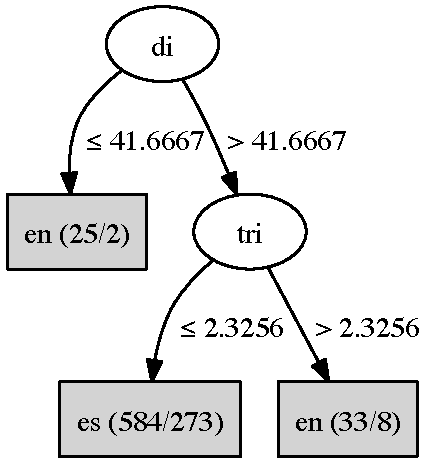
\includegraphics[width=1.5in]{c45-val.pdf}
\end{figure}

\begin{figure}[ht]
\centering
\caption{Lexical argument quantity C4.5 decision tree. The four attributes have values equal to the percentage of finite verbal clauses with zero, one, two, or three lexical arguments.}
\label{fig:c4.5-num-lex}
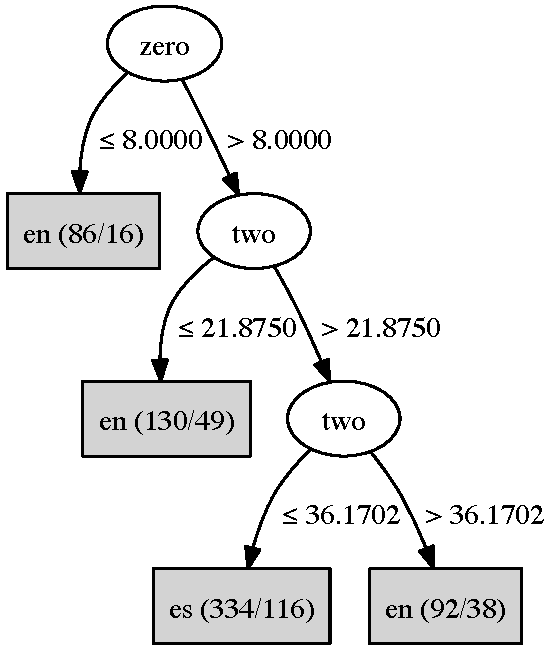
\includegraphics[width=2in]{c45-num-lex.pdf}
\end{figure}

\begin{figure}[ht]
\centering
\caption{Lexical argument role C4.5 decision tree. Attributes have values indicating the percentage of all lexical arguments which are found in that role.}
\label{fig:c4.5-lex-role}
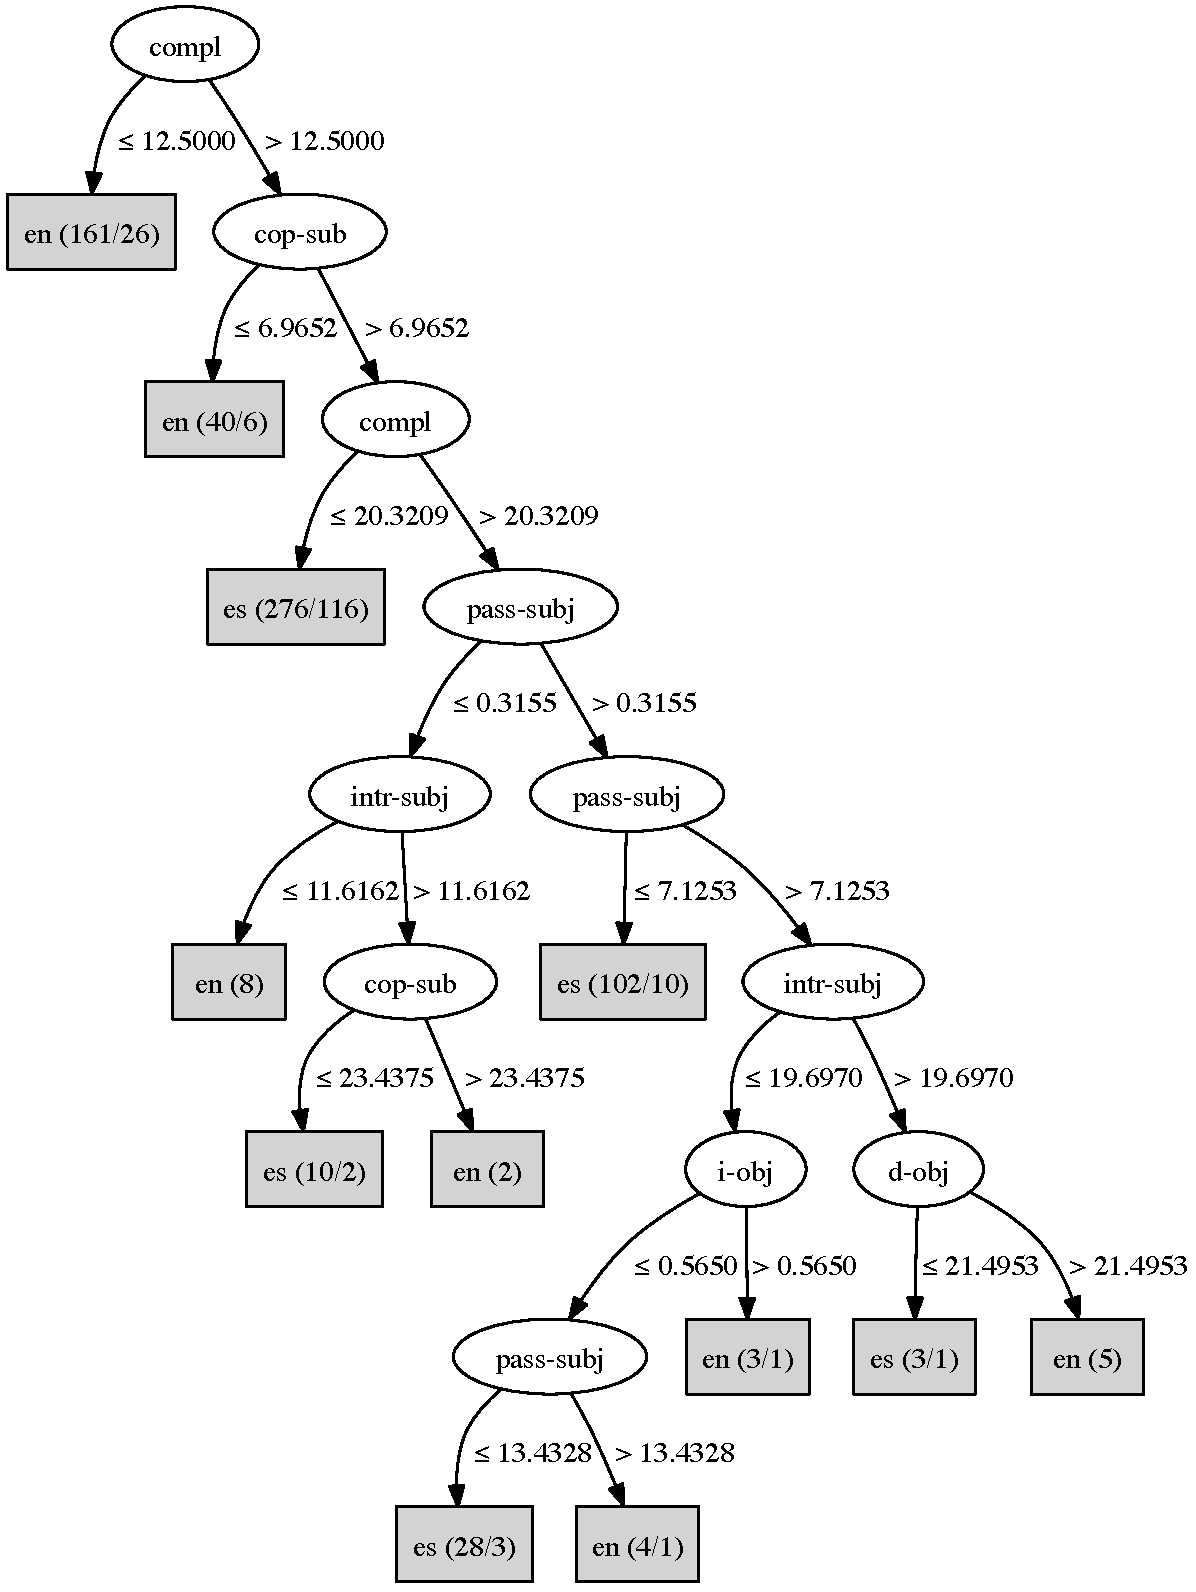
\includegraphics[width=4in]{c45-lex-role.pdf}
\end{figure}

\biblio
\end{document}